\subsection{Vue d'ensemble}
Un moteur d'exécution, ou {\em runtime}, est un morceau de logiciel utilisé par d'autres logiciels pour abstraire des parties du système.
%
L'idée principale est {\em compiler une fois, exécuter partout}.
%
Ils sont présent un peu partout et peuvent avoir différentes fonctions.
%
Certains langages dits de haut niveau utilisent un runtime, par exemple Java a un runtime pour gérer son ramasse-miettes.
%
Toutes les implémentations de MPI ont un runtime.
%
Les cadriciels de programmation à base de tâches tendent à utiliser un runtime.
%
Les parties suivantes se concentreront sur le support des runtimes pour la programmation à base de tâches.


Les runtimes utilisés pour la programmation à base de tâches doivent en premier lieu être capable d'ordonnancer le traitement des tâches tout en respectant l'ordre des dépendances entre les tâches (Fig.~\ref{fig:runtime}).
%
Ces runtime doivent aussi fournir un équilibrage de charge entre toutes les ressources matérielles disponibles (potentiellement hétérogènes) dans le but de minimiser le temps de calcul.
%
Certains runtimes s'occupent de transférer des données entre deux ressources potentiellement hétérogènes, comme par exemple entre la mémoire principale et la mémoire d'une carte graphique ou plus simplement entre deux processus.
%
Ces transferts peuvent être implicites, le runtime a connaissance des données qui sont manipulées, ou ils peuvent être explicites avec l'utilisation d'une tâche spéciale qui s'occupera de faire les échanges de données.

%   (-_-)   %
\begin{figure}
  \centering
  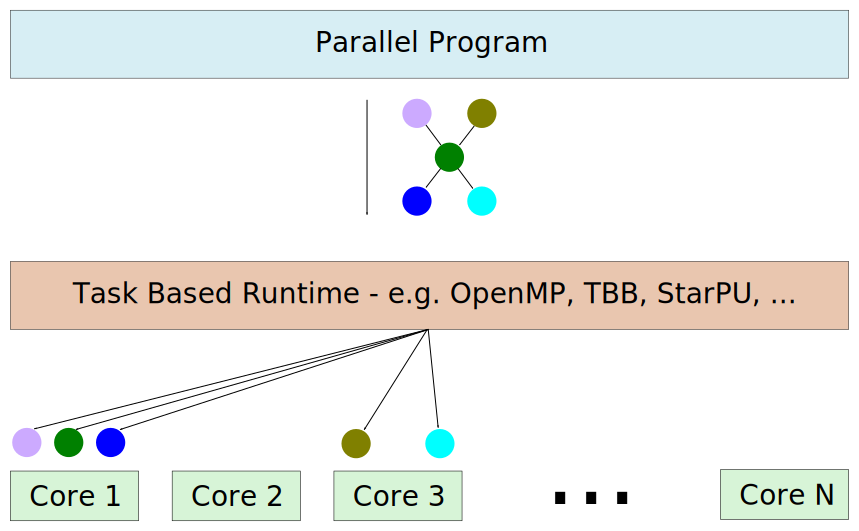
\includegraphics[width=0.8\textwidth]{runtime}
  \caption{Le programme parallèle fournit un graphe de tâches à l'ordonnanceur de tâches. Les tâches sont ensuite distribuées sur les coeurs de calcul disponibles.}
  \label{fig:runtime}
\end{figure}


Pour améliorer l'équilibrage de charge, les runtimes ont des politiques d'ordonnancement, la plupart de ces politiques sont dynamiques et peuvent s'adapter à la charge courante de la machine.
%
D'autres politiques d'ordonnancement, dîtes statiques, permettent de réduire le coût d'ordonnancement.
%
L'ordonnanceur parfait n'existe pas et n'existera sûrement jamais.
%
En effet, trouver le meilleur ordonnancement d'un ensemble de tâches avec un nombre limité de ressources de calcul est un problème NP-complet\footnote{Un problème est NP-complet si le temps nécessaire à la résolution du problèmes est polynomial comparé à la taille des données en entrées et que ce problème soit aussi difficile que tous les autres problèmes NP-complets.}.
%
Il existe des heuristiques d'ordonnancement qui donnent de bons résultats dans la majorité des cas, nous pouvons citer l'algorithme HEFT\cite{heft}.
%
Si le modèle de programmation le permet, des informations additionnelles peuvent être attribuées aux tâches, comme par exemple une estimation du temps de calcul, ces informations sont ensuite utilisées par l'ordonnanceur pour améliorer le placement des tâches.


L'apparition des premières machines parallèles à mémoire partagée a conduit à la recherche de nouvelles méthodes pour les programmer.
%
Il faut donc distribuer une charge de travail sur plusieurs unités de calcul.
%
Malheureusement, il arrive que cette charge de travail de soit pas connu l'avance.
%
Une idée est alors apparu pour rendre cette distribution plus flexible : le vol de travail (ou {\em work-stealing} en anglais).
%
Dès qu'une ressource de calcul n'as plus de travail, elle essaye de voler du travail à une autre ressource.
%
Le langage Cilk~\cite{Cilk}, apparu en 1994 et toujours développé sous le nom Cilk++~\cite{Cilk++}, permet de faire du vol de travail.
%
Les tâches sont décrites par le programmeur avec des mots clés additionnels au langage C, par exemple le mot-clé {\em spawn} placé avant l'appel d'une fonction permet à Cilk de comprendre qu'il doit créer une nouvelle tâche et qu'il doit l'ordonnancer.
%
Ces tâches sont empilées sur une pile spécifique à chaque thread.
%
Le vol de tâche se fait par le biais de cette pile de tâches (Fig.~\ref{fig:task_steal}).

%   (-_-)   %
\begin{figure}[t!]
  \centering
  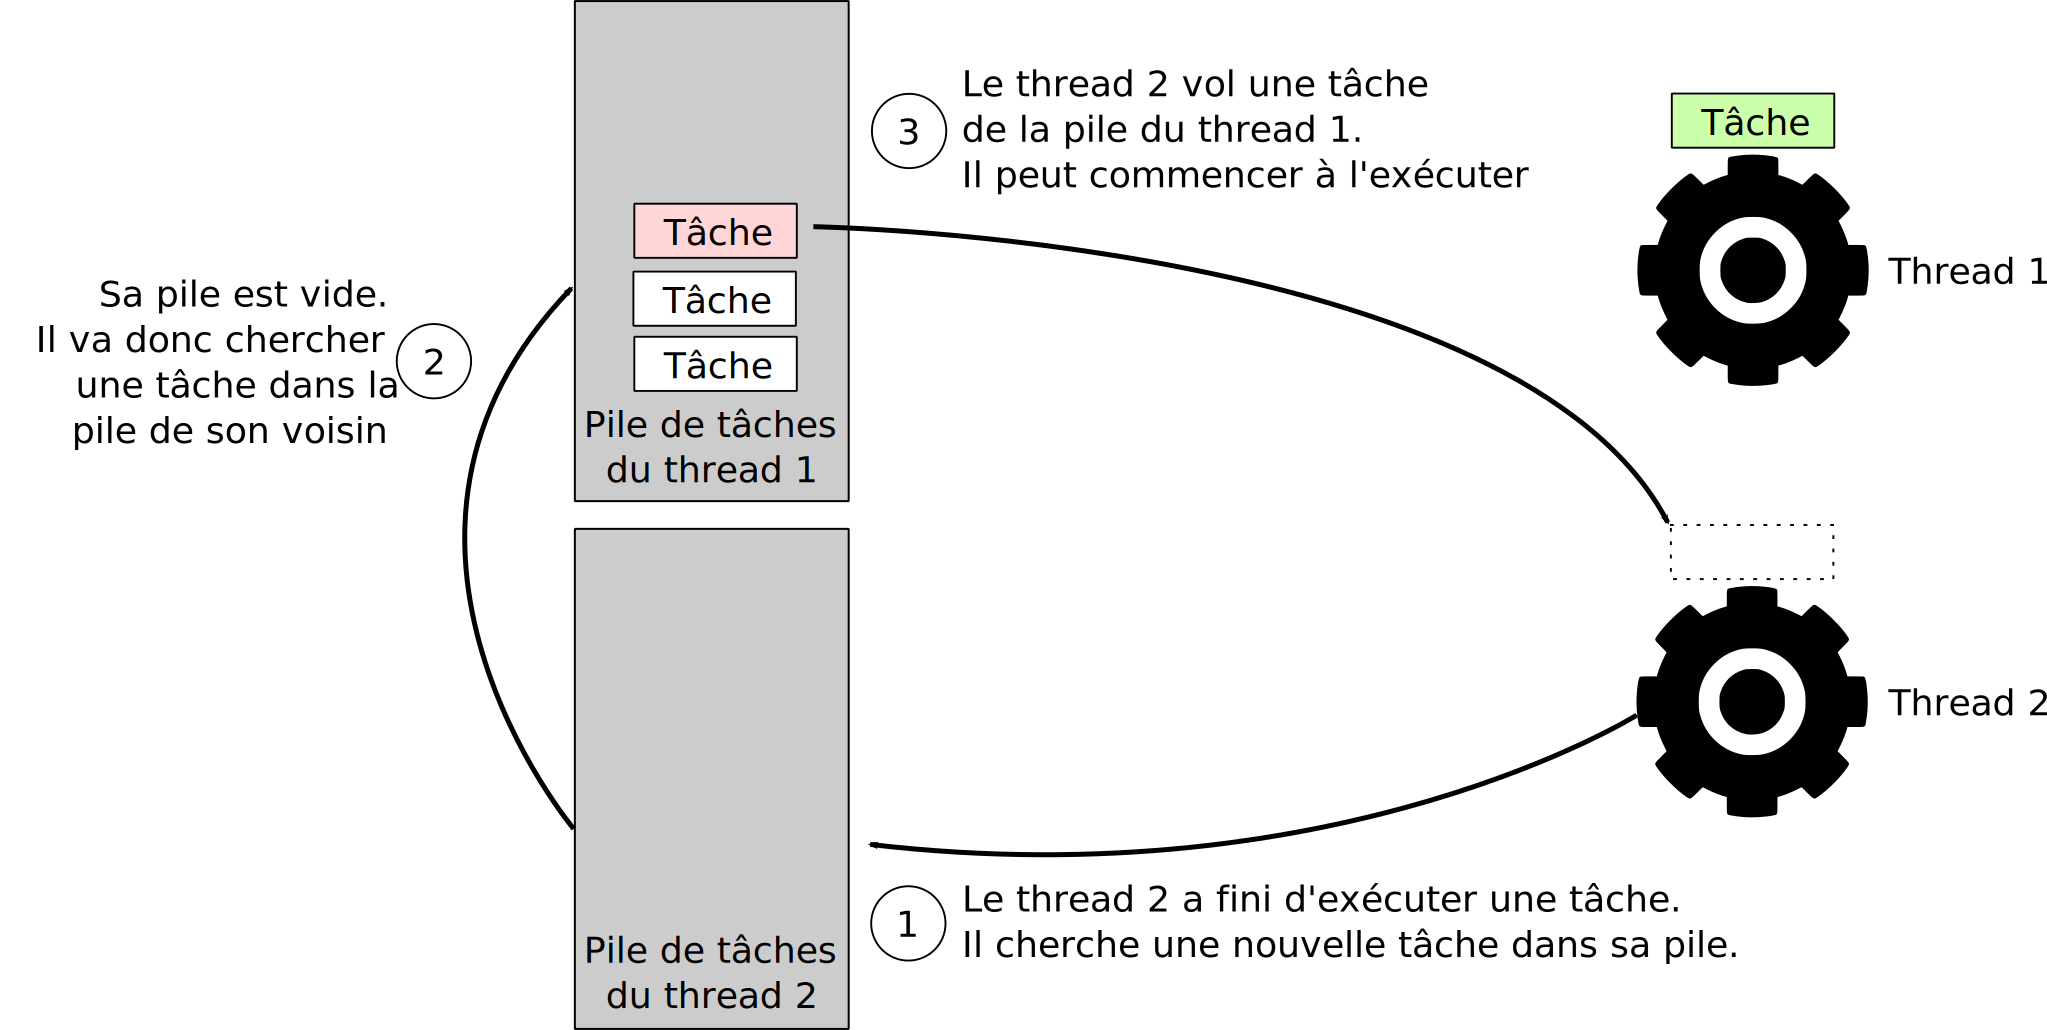
\includegraphics[width=\textwidth]{task_steal}
  \caption{Vol de tâche du thread 2 dans la pile du thread 1.}
  \label{fig:task_steal}
\end{figure}




Peu de temps après, en 1997, une interface de programmation parallèle voit le jour, il s'agit d'OpenMP~\cite{OpenMP}.
%
Les premières versions d'OpenMP se concentrent sur le parallélisme de boucle.
%
En ajoutant des annotations autour d'une boucle for, les itérations de la boucle seront distribuées sur les coeurs de calcul.
%
Il existe aussi des annotations permettant d'effectuer des réductions à la fin de la boucle.
%
Ce n'est qu'en 2008 que le support des tâches est ajouté à OpenMP dans sa version 3.0~\cite{openmptasks}.
%
Le programmeur peut créer des tâches parallèles mais il n'y a aucun moyen de spécifier les dépendances entre les tâches.
%
Les graphes de tâches ne peuvent donc pas être directement utilisés dans OpenMP.
%
OpenMP est donc un runtime très complet pour faire du parallélisme de boucle mais son modèle de tâches se rapproche du modèle de Cilk.


Intel TBB~\cite{Intel_TBB}, dont le développement a démarré en 2006, permet aussi de faire du parallélisme à base de tâches.
%
La gestion des dépendances entre les tâches est à la charge du programmeur mais TBB fournit les méthodes nécessaires telles que l'incrémentation et la décrémentation atomique du compteur de référence d'une tâche.
%
Le modèle d'abstraction du matérielle dans TBB ne permet pas de connaître le nombre de threads utilisés.
%
Ce choix est fait parce que pour Intel le programmeur n'a pas a se soucier des problèmes d'ordonnancement.




Plus récemment, à la fin des années 2000, la révolution du GPGPU donne lieu à l'apparition de nouveaux runtimes.
%
Les premières méthodes permettant d'utiliser un GPU pour du calcul étaient rudimentaires.
%
Il s'agissait de détourner l'utilisation des shaders programmables des interfaces de programmation graphiques comme par exemple OpenGL.
%
Puis des langages spécifiques ont vus le jour, parmi ceux ci, les plus populaires sont CUDA et OpenCL.
%
CUDA est développé par NVidia et ne permet de programmer que des GPU NVidia.
%
OpenCL est une spécification du Khronos Group et a pour but de fournir une interface de programmation standard pour programmer toutes sortes d'accélérateurs.
%
Ces accélérateurs peuvent être des GPUs mais de manière générale il s'agit de co-processeurs déportés.



StarPU~\cite{starpu}, développé à Inria permet de d'écrire plusieurs versions d'une routine à la fois pour le CPU et le GPU.
%
Ces morceaux de codes spécifiques à une architecture sont appelés {\em codelets}.
%
Puis les stratégies d'ordonnancement intégrées à StarPU choisiront la codelet qui permettra d'obtenir le meilleur temps de calcul.
%
Ce choix prend aussi en compte le temps de transfert mémoire entre la mémoire centrale et la mémoire du GPU.
%
Pour avoir une gestion efficace de ces transferts mémoires, StarPU implémente un gestionnaire mémoire.
%
Ce gestionnaire est capable d'effectuer des transferts entre toutes les zones mémoires de la machine (mémoire centrale, mémoire GPU, disques, ...) et de maintenir la cohérence des données.
%
Par exemple, si une donnée A est en mémoire centrale et qu'une codelet doit l'utiliser sur le GPU, il y aura d'abord une copie A vers la mémoire du GPU.
%
Ensuite tant que cette donnée n'est accédée qu'en lecture, il y aura deux copies valides, une en mémoire centrale et une en mémoire GPU.
%
Dès qu'une codelet accède à la donnée en écriture, toutes les autres copies sont invalidées et un transfert mémoire sera nécessaire pour les mettre à jour.
%
StarPU intègre aussi plusieurs politiques d'ordonnancement permettant d'adapter à plusieurs code de calcul.
%
L'équipe de développement met aussi en avant la possibilité d'écrire son propre ordonnanceur et de l'intégrer à StarPU.


X-KAAPI~\cite{xkaapi} est aussi développé à Inria et permet de programmer des applications qui auront du code qui sera exécuté à la fois sur CPU et sur GPU.
%
Il se différencie de StarPU par son système de vol de tâches dynamique.
%
X-KAAPI va partitionné le graphe de tâches et distribuer les partitions aux threads.
%
Chaque thread a ainsi une première approximation de l'ordonnancement du graphe.
%
Le surcoût de gestion des dépendances est ainsi limité aux frontières entre les partitions.
%
Lors de l'exécution du code, si un thread se retrouve à court de tâches, il va essayer d'en voler à un autre thread que l'on appellera {\em victime}.
%
Mais il ne va pas la voler complètement, il la laisse dans la pile de la victime en ajoutant comme information que la tâche a été volée.
%
Ainsi lorsque la victime découvrira qu'une tâche a été volée, elle devra vérifier les dépendances de cette tâche.
%
Ce système permet de réduire le surcoût d'ordonnancement, avec un bon partitionnement, le vol de tâche est plus rare et beaucoup de temps a été économisé sur la gestion des dépendances.



OmpSs~\cite{OMPSs} est un runtime qui permet, tout comme StarPU et X-KAAPI, d'écrire du code à la fois pour le CPU et pour le GPU puis de laisser le runtime choisir parmi toutes les versions d'une fonction.
%
La différence entre ces deux runtimes provient surtout de la description du parallélisme.
%
OmpSs propose un approche à base d'annotation de code en étendant la spécification OpenMP version 3.
%
Cette extension permet au mot clé {\em task} d'être accompagné d'informations complémentaires sur l'utilisation des paramètres en entrée.
%
OmpSs pourra ensuite déduire les dépendances entre les tâches depuis les informations sur les paramètres en entrée.
%
Il n'y a pas non plus d'écriture automatisée de code, le programmeur doit toujours écrire le code spécifique à chaque architecture précédé d'informations concernant la fonction implémentée ainsi que l'architecture cible.


HMPP~\cite{hmpp} est un runtime, développé par CAPS, adressant le problème de la programmation hybride CPU/GPU.
%
Il s'utilise avec des annotations de code de la même manière qu'OpenMP et qu'OmpSs.
%
Puis le code annoté est ensuite transformé par un compilateur source-to-source vers un autre langage spécifique à l'architecture cible, comme le CUDA par exemple.
%
Les transferts mémoires entre la mémoire centrale et la mémoire du GPU peuvent être fait de deux façons :
\begin{itemize}
  \item implicitement au moment de l'appel de la codelet mais cette méthode ne permet de recouvrir la communication par du calcul;
  \item explicitement avec l'ajout d'annotation, il est donc à la charge du programmeur de choisir le bon moment pour transférer les données.
\end{itemize}
%



OpenACC~\cite{OpenACC} est un standard de programmation développé par un consortium de société dans le but de simplifier la programmation parallèle hybride CPU/GPU.
%
Les spécificités de ce standard ressemble en de nombreux points à HMPP (annotations, gestion mémoire, ...).
%
Son principal avantage est qu'il est soutenu par plusieurs sociétés là où HMPP n'est plus supporté.
%
OpenMP ajoute dans version 4 le support de la programmation hybride, son fonctionnement est identique à OpenACC, seuls les mot-clés changent.


PaRSEC~\cite{PaRSEC} est un runtime développé à l'ICL permettant de travailler directement en mémoire distribuée.
%
Le parallélisme dans PaRSEC doit être décrit dans un langage spécifique, le JDF.
%
L'ensemble des tâches du programme est décrit dans ce langage et ce n'est que la distribution des données en mémoire distribuée qui détermineras le processus qui exécuteras la tâche.
%
PaRSEC s'occupe automatiquement des communications entre processus permettant de maintenir une cohérence entre les données.
%
L'inconvenient majeur de ce runtime est son manque de flexibilité.
%
Le format JDF ne permet de créer dynamiquement de nouvelle tâche.
